% !TeX spellcheck = en_US
% !TeX encoding = utf8
% !TeX program = xelatex
% !BIB program = bibtex

\documentclass[12pt]{article}
	\usepackage{amsmath,amssymb,amsfonts}
	\usepackage{hyperref}
	\usepackage{latexsym}
	\usepackage{graphicx}
	\usepackage{verbatim}
	\usepackage{booktabs}
	\usepackage[usenames,dvipsnames,svgnames,table]{xcolor}
	\usepackage{todonotes} % Required for the boxes that questions appear in
	\usepackage{mmstyles}
	\newcommand{\mybox}[1]
	{
	\par\noindent
	\todo[inline, backgroundcolor=SkyBlue!40,bordercolor=SkyBlue,size=\large]{\textbf{#1}}
	
	}

	\usepackage[top=25mm, bottom=25mm, left=18mm, right=18mm]{geometry}

	% \usepackage{fancyhdr}
	% \pagestyle{fancy}
	% \lhead{Linear Optimization Assignment \#3}
	% \chead{}
	% \rhead{Due: Friday, May 4 (Tentative)}
	% \renewcommand{\headrulewidth}{0.3pt}

	% \usepackage[framed,numbered,autolinebreaks,useliterate,final]{mcode}
	\usepackage{listings}
	\title{\textbf{ Homework3: Convolutional Arithmetic \\ Supplementary Material  }}
	\author{}
	\date{}

	% \makeatletter
	% \def\@seccntformat#1{%
	% 	\expandafter\ifx\csname c@#1\endcsname\c@section\else
	% 	\csname the#1\endcsname\quad
	% 	\fi}
	% \makeatother

	\usepackage{multirow}
	\usepackage{sectsty}
	\usepackage{fontspec}
	\usepackage[slantfont,boldfont]{xeCJK}
	% \sectionfont{\color{NavyBlue}\selectfont}
	% \subsectionfont{\color{SkyBlue}\itshape\selectfont}
	\usepackage{nicefrac}
	\newcommand{\pp}[2]{\nicefrac{\partial #1}{\partial #2}}
	\newcommand{\fpp}[2]{\frac{\partial #1}{\partial #2}}
	\newcommand{\abs}[1]{\left| #1 \right| }
	\newcommand{\norm}[1]{\left\| {#1} \right\|}
	\newcommand{\red}[1]{{\color{red}{#1}}}
	\usepackage{titlesec,titletoc} 
	\renewcommand*{\thesection}{\color{NavyBlue}Problem \arabic{section} } 
	\renewcommand*{\thesubsection}{\color{SkyBlue}Solution \arabic{section} } 
	\titleformat{\section}[hang]{\bfseries}{\thesection}{1em}{}{}
	\titleformat{\subsection}[hang]{\itshape}{\thesubsection}{1em}{}{}
	
	% \setlength{\parsep}{0em}
	% \setlength{\itemsep}{0pt}
	\setlength{\parskip}{.33em}
	\setlength{\parindent}{0em}	

	\providecommand{\tightlist}{%
	\setlength{\itemsep}{0pt}\setlength{\parskip}{0pt}}
  
\begin{document}
% \vspace{-1em} 
\maketitle

\paragraph{前向传播} test
% $$(I * K)_{ij} = (I \otimes \text{rot}_{180^\circ}\{K\} )_{ij}$$
考虑卷积核输入通道数目为1,个数为1的情况。此时,卷积运算表达式为:
$$x_{i,j}^l = \sum_{m}\sum_{n} w_{m,n}^l x_{i + m,j + n}^{l-1} + b^l$$
其中$\mX^{l-1} = (x^{l-1})_{ij}$表示当前层的输入,$\mX = (x^l)_{ij}$表示当前层的输出。

卷积神经网络中的卷积运算事实上为Cross Correlation运算($\otimes$),
$$x_{i,j}^l = \left\{ w_{m,n}^l \right\} \otimes x_{i,j}^{l-1} + b_{i,j}^l $$
或者可以理解为卷积核反褶后的卷积运算($*$)
$$x_{i,j}^l = \text{rot}_{180^\circ} \left\{ w_{m,n}^l \right\} \ast x_{i,j}^{l-1} + b_{i,j}^l $$

\paragraph{反向传播}

对输入的梯度和对卷积核的梯度为
\begin{align}
	\delta  w_{m^{\prime},n^{\prime}}^l & = \delta x^{l}_{i,j} \otimes x_{m^{\prime},n^{\prime}}^{l-1}                                                                  \\
	\delta x_{i',j'}^{l-1}              & =  \delta x^{l}_{i',j'} \ast   w_{m,n}^{l} = \delta x^{l}_{i',j'} \otimes \text{rot}_{180^\circ} \left\{ w_{m,n}^{l} \right\}
\end{align}

\subparagraph{举例}
对于
\begin{equation}
	\begin{bmatrix}
		O_{11} & O_{12} \\
		O_{21} & O_{22}
	\end{bmatrix} =
	\begin{bmatrix}
		X_{11} & X_{12} & X_{13} \\
		X_{21} & X_{22} & X_{23} \\
		X_{31} & X_{32} & X_{33}
	\end{bmatrix}
	\otimes
	\begin{bmatrix}
		W_{11} & W_{12} \\
		W_{21} & W_{22}
	\end{bmatrix}
\end{equation}
其中$\mO$表示当前层的输出,$\mX$表示上一层的输入。

目标函数对$O$的梯度为
\begin{equation}
	\begin{bmatrix}
		\pp{E}{W_{11}} & \pp{E}{W_{12}} \\
		\pp{E}{W_{21}} & \pp{E}{W_{22}}
	\end{bmatrix} =
	\begin{bmatrix}
		X_{11} & X_{12} & X_{13} \\
		X_{21} & X_{22} & X_{23} \\
		X_{31} & X_{32} & X_{33}
	\end{bmatrix}
	\otimes
	\begin{bmatrix}
		\pp{E}{O_{11}} & \pp{E}{O_{12}}  \\
		\pp{E}{O_{21}} & \pp{E}{O_{22} }
	\end{bmatrix}
\end{equation}

目标函数对卷积核的梯度为
\begin{equation}
	\begin{bmatrix}
		\pp{E}{X_{11}}  & \pp{E}{X_{12}}  & \pp{E}{X_{13}}  \\
		\pp{E}{X_{21} } & \pp{E}{X_{22}}  & \pp{E}{X_{23}}  \\
		\pp{E}{X_{31} } & \pp{E}{X_{32} } & \pp{E}{X_{33} }
	\end{bmatrix} =
	\begin{bmatrix}
		\pp{E}{O_{11}} & \pp{E}{O_{12}}  \\
		\pp{E}{O_{21}} & \pp{E}{O_{22} }
	\end{bmatrix}
	\otimes
	\begin{bmatrix}
		W_{22} & W_{21} \\
		W_{12} & W_{11}
	\end{bmatrix}
\end{equation}
此处,padding方式应该为`full'。如图~\ref{fig:full}所示。

\begin{figure}
	\centering
	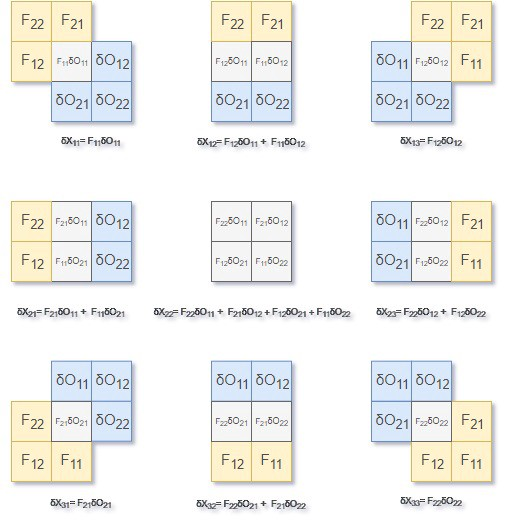
\includegraphics[width=.8\textwidth]{fig/2018-04-24-19-27-44.png}
	\caption{padding方式应该为`full',其中$\mF$表示权重} \label{fig:full}
\end{figure}

\subparagraph{证明}

\begin{align}
	\delta  w_{m^{\prime},n^{\prime}}^l = \frac{\partial E}{\partial w_{m^{\prime},n^{\prime}}^l} & = \sum_{i=0}^{H-k_1} \sum_{j=0}^{W-k_2} \frac{\partial E}{\partial x_{i,j}^{l}} \frac{\partial x_{i,j}^{l}}{\partial w_{m^{\prime},n^{\prime}}^l} \\
	                                                                                              & = \sum_{i=0}^{H-k_1} \sum_{j=0}^{W-k_2} \delta x^{l}_{i,j} \frac{\partial x_{i,j}^{l}}{\partial w_{m^{\prime},n^{\prime}}^l}
\end{align}

其中\begin{align}
	\frac{\partial x_{i,j}^{l}}{\partial w_{m^{\prime},n^{\prime}}^l} & = \frac{\partial}{\partial w_{m^{\prime},n^{\prime}}^l}\left( \sum_{m} \sum_{n} w_{m,n}^{l}x_{i+m, j+n}^{l-1} + b^l \right)                                              \\
	                                                                  & = \frac{\partial}{\partial w_{m',n'}^l}\left( w_{0,0}^{l} x_{ i + 0, j + 0}^{l-1} + \dots + w_{m',n'}^{l} x_{ i + m^{\prime}, j + n^{\prime}}^{l-1} + \dots + b^l\right) \\
	                                                                  & = \frac{\partial}{\partial w_{m^{\prime},n^{\prime}}^l}\left( w_{m^{\prime},n^{\prime}}^{l} x_{ i + m^{\prime}, j + n^{\prime}}^{l-1}\right)                             \\
	                                                                  & =  x_{i+m^{\prime},j+n^{\prime}}^{l-1}
\end{align}

因此\begin{align}
	\delta  w_{m^{\prime},n^{\prime}}^l = \frac{\partial E}{\partial w_{m',n'}^l} & = \sum_{i=0}^{H-k_1} \sum_{j=0}^{W-k_2} \delta^{l}_{i,j} x_{ i + m^{\prime}, j + n^{\prime}}^{l-1} \\
	                                                                              & = \delta x^{l}_{i,j} \otimes x_{m^{\prime},n^{\prime}}^{l-1}                                       \\
	                                                                              & = \text{rot}_{180^\circ} \left\{ \delta x^{l}_{i,j} \right\} \ast  x_{m^{\prime},n^{\prime}}^{l-1}
\end{align}

同理\begin{align}
	\delta x_{i',j'}^{l-1} & = \sum_{m = 0}^{k_1 - 1} \sum_{n = 0}^{k_2 - 1} \delta x^{l}_{i^{\prime} - m,j^{\prime} - n} w_{m,n}^{l} \\
	                       & =  \delta x^{l}_{i',j'}*   w_{m,n}^{l}                                                                   \\
	                       & = \delta x^{l}_{i',j'} \otimes \text{rot}_{180^\circ} \left\{ w_{m,n}^{l} \right\}
\end{align}

\paragraph{Max Pooling}

如果$f(\vx)=\max(x_1,x_2)$,则$\fpp{f}{\vx} = \begin{cases}
	(1,0)^T &, x_1 > x_2 \\
	(0,1)^T & ,x_1 < x_2 \\
	\alpha (1,0)^T + (1-\alpha) (0,1)^T &, x_1 = x_2
\end{cases}$

可见,梯度反传到最大值处即可。

\paragraph{举例}

\begin{equation}
	\begin{bmatrix}
		\begin{bmatrix}
			\red{5} & 3 \\
			1 & 2 
		\end{bmatrix} &
		\begin{bmatrix}
			1 & 2 \\
			\red{3} & 2 
		\end{bmatrix} \\ \\
		\begin{bmatrix}
			4 & 2 \\
			3 & \red{6} 
		\end{bmatrix} & 
		\begin{bmatrix}
			2 & \red{5} \\
			1 & 1 
		\end{bmatrix} 
	\end{bmatrix} \rightarrow 
	\begin{bmatrix}
		5 & 3 \\
		6 & 5 
	\end{bmatrix}
\end{equation}

\begin{equation}
	\begin{bmatrix}
		\begin{bmatrix}
			\red{1} & 0 \\
			0 & 0 
		\end{bmatrix} &
		\begin{bmatrix}
			0 & 0 \\
			\red{.8} & 0 
		\end{bmatrix} \\ \\
		\begin{bmatrix}
			0 & 0 \\
			0 & \red{.4} 
		\end{bmatrix} & 
		\begin{bmatrix}
			0 & \red{.6} \\
			0 & 0 
		\end{bmatrix} 
	\end{bmatrix} \leftarrow 
	\begin{bmatrix}
		1 & .8 \\
		.4 & .6 
	\end{bmatrix}
\end{equation}

\end{document}

